\section{General class of models}
Let us consider $(r, \F, \F_{t}, \Pbb)$, 
$W_{t} \left\lbrace W_{t}^{1}, \cdots, W_{t}^{d} \right\rbrace$,
$\F_t = \sigma \left\lbrace W_u: u \leq t \right\rbrace$
\begin{rem}
 Where \Pbb is what is termed \textit{the historical measure}
\end{rem}
\begin{itemize}
 \item Short rate $\left\lbrace r(t): t \geq 0 \right\rbrace$ such that 
\begin{equation}
 r(t) = r(0) + \int_{0}^{t} b(s) ds + \int_0^t \sigma(s) dW_{s}
\end{equation}
Were both $b \text{ and } \sigma$ are $\F_t$ - progressive measurable processes. 
And $dW_s$ is a d-dimension \textit{Brownian Motion}(B.M.)
We assume that $\int_0^T \left( |b(s)| + \|\|^2_{\Rbb_{d}}\right) < + \infty$ a.s. $\forall \text{T}$
\item $\exists \Qbb \cong \Pbb$ such that $\dfrac{d \Qbb}{d \Pbb} = \exp \left\lbrace\int_0^\infty \gamma(s) dW_s
- \dfrac{1}{2} \int_0^\infty \gamma^{2}(s) ds \right\rbrace$ 
\newline Where $\gamma(s)$ is a $\F_t$ - progressive measurable process, and the above integrals are
of Girasnov type and satisfy the Novikov condition is a ($\F_t, \Qbb$)-martingale in $[0,T]$ $\forall T 
\lt +\infty$
\begin{equation}
 \dfrac{P(t,T)}{S_{0}(t)} = \dfrac{P(t,T)}{\exp(\int_0^t r(s) ds}
\end{equation}
where $S_0(t)$ is the Money Market Account, and $P(t,T)$ price in t of a zero-coupon bond with maturity T
\end{itemize}
$\Qbb$ is an equivalent \textit{Martingale Measure}(M.M) for the model, and this implies the \textbf{First
 Fundamental
Theorem of Arbitrage} 
\begin{thm}
 Every restricted market ($P(\cdot, T_1); \cdots ; P(\cdot, T_m), S_{0}(t)$) m-finite is \textit{arbitrage free}
\end{thm}
We can derive the fundamental relation 
$\dfrac{P(t,T)}{S_0(t)} = \mathbb{E}_{\Qbb} \left\lbrace \dfrac{1}{S_{0}(T)} | \F_{t}\right\rbrace$
\footnote{$P(T,T) = 1$}
$\Rightarrow P(t,T) = \mathbb{E}_{\Qbb} \left\lbrace e^{-\int_{0}^{T} r(s) ds} | \F_t\right\rbrace$
\begin{dfn}
The short rate, $r_t \,$, is the (continuously compounded, annualized) interest rate at 
which an entity can borrow money for an infinitesimally short period of time from time t. 
Specifying the current short rate does not specify the entire yield curve. However
 arbitrage arguments show that, under some fairly relaxed technical conditions, 
if we model the evolution of $r_t \,$ as a stochastic process under a risk-neutral measure $\Qbb$ 
then the price at time t of a zero-coupon bond maturing at time T is given by

:$ P(t,T) = \mathbb{E}\left[\left. \exp{\left(-\int_t^T r_s\, ds\right) } \right| \mathcal{F}_t \right] $

where $\mathcal{F}$ is the natural filtration for the process.

\end{dfn}
\subsection{Dynamics of Short Rate Models}
We will consider $t \Rightarrow P(t,T)$ (under \Pbb, under \Qbb)
\begin{enumerate}
 \item Due to Girasnov's Theorem $W_t - \int_0^t \gamma(s) ds =: W_t^{*}$ is a 
$(\Qbb, \F_t)$- d-dimensional Brownian Motion. So: $dr_t = r(0) + \int_0^t \sigma(s) dW^{*}_s + 
\int_0^t (b_s + \sigma(s) \gamma^{T} (s)) ds$
\newline Note that $dW^{*}_s = dW_s - \gamma^{T}(s)ds$ and looking at 
$\int_0^t (b_s + \sigma(s) \gamma^{T} (s)) ds$ we see that the drift has changed.
\item For every $T \lt +\infty$ $\exists \F_t$-progressive process $\left\lbrace v(t,T): t \leq T \right\rbrace$ 
such that $\dfrac{d \Pbb(t,T)}{P(t,T)} = r(t)dt + v(t,T) dW^*_t$
\newline 
\textbf{Indeed} P(t,T) = $e^{\int_{)}^{t}r(s)ds} \mathbb{E}_{\Qbb}\left\lbrace \dfrac{1}{S_{0}(T)}| \F_t
\right\rbrace = e^{\int_{0}^{t}r(s)ds}M_t^{(T)}$ since $M_t^{(T)}$ is a $(\Qbb, \F_t)$-martingale, $\exists \F_t$
-progressive process ($t \leq T)$ $\left\lbrace h(t,T): t \leq T\right\rbrace$ such that $M_t^{(T)} = M_0^{(T)} +
\int_{0}^{t} h(s,T)dW^*_s $
where $\left\lbrace h(t,T): t \leq T\right\rbrace$ is  a d-dimensional object.
\newline 
d\Pbb(t,T) = d $\left\lbrace e^{\int_{0}^{T}r(s)ds} \times M^{(T)}_t\right\rbrace = M^{(T)}_t d\left\lbrace
e^{\int_{0}^{T}r(s)ds} \right\rbrace + e^{\int_{0}^{T}r(s)ds} dM^{(T)}_{t}$
\begin{displaymath} =P(t,T) r(t)dt + e^{\int_{0}^{T}r(s)ds}
h(t,T) dW^*_t = P(t,T)r(t) dt + P(t,T) v(t,T) dW^*_{t} \end{displaymath}
with $v(t,T) = \dfrac{e^{\int_{0}^{T}r(s)ds}h(t,T)}{P(t,T)}$
\newline As a consequence we can say 
$P(t,T) = P(0,T)\exp{\int_0^t r(s) ds + \int_0^t v(s,T)dW^*_s - \frac{1}{2} \int_0^t v^{2} (s,T) ds}$
$= P(0,T) S_{0}(t) Z_{t}^{(T)}$, where 
$Z_{t}^{(T)}:=\exp{\int_0^t r(s) ds + \int_0^t v(s,T)dW^*_s - 
\frac{1}{2} \int_0^t v^{2} (s,T) ds}$ can be thought of as a 'pertubation' of a 'time series' 
and is also an $\F_t$-martingale under \Qbb
Also $\dfrac{P(t,T)}{S_{0}(t)} = P(0,T)Z_{t}^{(T)} := \tilde{P}(t,T)$
$\dfrac{d\tilde{P}(t,T)}{\tilde{P}(t,T)} = v(t,T) dW_t^{*}$
\item Under \Pbb? 
\begin{equation}
 \dfrac{d \Pbb(t,T)}{\Pbb(t,T)} = r(t)dt + v(t,T) dW_t^{*} 
\end{equation}
Note: $dW_t^{*} = \left\lbrace dW_t - \gamma^{T} (t) dt\right\rbrace$
= $\underbrace{\left\lbrace r(t) - v(t,T) \gamma^{T}(t) \right\rbrace}_{\text{:=$\alpha$(t,T)}} dt + v(t,T)dW_{t}$
\end{enumerate}
P(t,T) = $P(0,T)\exp{\int_{0}^{t} \alpha(t,T)ds + \int_0^t v(s,T) dW_s -\frac{1}{2} \int_0^t v(s,T)^{2}ds}$
$$\tilde{P}(t,T) = P(0,T) \exp{-\int_0^t v(s,T)}\gamma^{T}(s)ds + \int_0^t v(s,T) dW_s - \frac{1}{2} \int_0
^t v(s,T)^{2} ds$$
\begin{rem}
 Recall $-\gamma= \text{Market Price of Risk}$
\end{rem}
\subsection{Short rate diffusions}
Let us consider Short rate diffusions 
$(\Omega, \F_t, \Pbb); \underbrace{\Qbb}_{\gamma}, d=1, W_t = \left\lbrace W_t: t \geq 0\right\rbrace$
\textbf{Assume} \begin{equation}\label{dagger}
                 \forall s \geq 0 
\begin{cases} dr_{t}=b(t,r_{t})dt + \sigma(t,r_{t})dW^{*}_{t}  \\ 
r_{0} = \text{constant}
\end{cases} 
                \end{equation}
with values in Z $\Rbb$ or $\Rbb_{+}$.
Take $b, \sigma$ to be Lipschitz formulas
Before proceeding let us recall what a Lipschitz Function is
\begin{dfn}
 Given two \textit{metric space}s (X, d$_X$) and (Y, d$_Y$), where d$_X$ 
denotes the \textit{metric} on the set X and d$_Y$ is the metric on set Y (for example, Y might be the set of 
\textit{real numbers} \Rbb 
with the metric d$_Y$(x, y) = |x − y|, and X might be a subset of \Rbb), a function 
\begin{displaymath}\displaystyle f: X \to Y\end{displaymath} 
is called 'Lipschitz continuous' if there exists a real constant K ≥ 0 such that, for all x$_1$ and x$_2$ in X,
\begin{displaymath} d_Y(f(x_1), f(x_2)) \le K d_X(x_1, x_2).\end{displaymath}
Any  such K is referred to as  'a Lipschitz constant' for the function f. 
The smallest constant is sometimes called \textbf{the (best) Lipschitz constant}; 
however in most cases the latter notion is less relevant. 
If K = 1 the function is called a	\textit{short map}, 
and if $0 \leq K \leq 1$ the function is called a \textit{contraction mapping}.

The inequality is (trivially) satisfied if x$_1$ = x$_2$. Otherwise, one can equivalently 
define a function to be Lipschitz continuous 			\textit{if and only if} 
there exists a constant K $\geq$ 0 such that, for all x$_1$ $\neq$ x$_2$,  
\begin{displaymath}\frac{d_Y(f(x_1),f(x_2))}{d_X(x_1,x_2)}\le K.\end{displaymath}
For real-valued functions of several real variables, this holds if and only 
if the absolute value of the slopes of all secant lines are bounded by K.  
The set of lines of slope K passing through a point on the graph of the function forms a circular cone,
 and a function is Lipschitz if and only if the graph of the function everywhere lies completely outside
 of this cone.

A function is called 'locally Lipschitz continuous' if for every x in X there exists a 	
\textit{neighborhood} U of x such that f restricted to U is Lipschitz continuous.  
Equivalently, if X is a \textit{locally compact} metric space, then f is locally Lipschitz 
if and only if it is Lipschitz continuous on every compact subset of X. 
 In spaces that are not locally compact, this is a necessary but not a sufficient condition.

More generally, a function f defined on X is said to be 'Hölder continuous' or to satisfy a 			
\textit{Hoelder condition} of order $\alpha > 0$on X if there exists a constant M > 0 such that
\begin{displaymath}\displaystyle d_Y(f(x), f(y)) \leq M d_X(x,  y)^{\alpha}\end{displaymath} 
for all x and y in X. Sometimes a Hölder condition of order α is also called a 'uniform Lipschitz 
condition of order' $\alpha > 0$.

If there exists a $K \geq 1$ with
\begin{displaymath}\frac{1}{K}d_X(x_1,x_2) \le d_Y(f(x_1), f(x_2)) \le K d_X(x_1, x_2)\end{displaymath}
then ƒ is called 'bilipschitz' (also written 'bi-Lipschitz').  A bilipschitz mapping is 
\textit{injective function}, and is in fact a 			
\textit{homeomorphism} onto its image.  A bilipschitz function is the same thing as an 
injective Lipschitz function whose 			
\textit{inverse function} is also Lipschitz. 
 Surjective bilipschitz functions are exactly the isomorphisms of metric spaces.
\end{dfn}
\subsection{How do we relate P(t,T) to a PDE}
In Financial Modelling there are said to be two main approaches, the 'martingale' approach and the PDE approach.
We know for example that the Black Scholes equation is a Parabolic PDE. Thanks to some of the theorems that one 
encounters in a good PDE Lecture Course or in a textbook, there is a range of techology to solve PDEs. 
 This is not a 'PDE and analysis' course, so we won't venture too far into the study of PDE, but we will
make some remarks about how these PDEs are solved. 
\begin{align}
 \text{Let T be fixed} P(t,T) = \mathbb{E}_{\Qbb}\left[\left. \exp{\left(-\int_t^T r(s)\, ds\right) } \right| 
\mathcal{F}_t \right] \stackrel{=}{\text{Markov Property of SDE}} \\
\mathbb{E}_{\Qbb} \left[ \exp{\left(-\int_t^T r(s)\, ds\right) } | r_{t}\right] = F(t,r_{t}
\end{align}
For some function $F(\cdot, \cdot)$ deterministic with random arguments, with 
\begin{displaymath}
F(t,x) =: \mathbb{E}_\Qbb \left\lbrace \exp\left(-\int_t^T r(s)\, ds\right)  |r_{t} =x\right\rbrace 
\end{displaymath}
\begin{thm}
 Fix T $\gt$ 0, and adopt the previous notation. Assume that
$F:[0,T] \times Z$ with $\Theta: Z \rightarrow \Rbb_{+}$is a solution of 
\begin{equation}\label{pde}
\begin{cases}
 \dfrac{\partial F}{\partial t} (t,r) + b(t,r) \dfrac{\partial}{\partial r} F(t,r) + \dfrac{1}{2} \sigma^{2}
(t,r) \dfrac{\partial^{2}}{\partial r^{2}} F(t,r) = rF(t,r) \\
F(T,r) = \Theta(r)
\end{cases}
\end{equation}

\textbf{Then:} $t \Rightarrow M_{t}:= F(t,r_{t})\exp{-\int_{0}^{t}r(s)ds}$ is a $(\F_t, \Qbb)$- local martingale
on [0,T]. If moreover: 
either 

\begin{enumerate}\label{check}
 \item $M_t$ is u.i. or 
\item $\mathbb{E}_{\Qbb}\left[ \int_0^T 
\left(\partial_{r} F(t, r_{t}\right)\exp{-\int_{0}^{t}r(s)ds}\sigma(t, r_{t}))^{2}dt\right]$

\end{enumerate}

Then $F(t, r_{t}) = \mathbb{E}_{\Qbb}(M_{T} | \F_t) = \mathbb{E}_{\Qbb} \left[F(T,r_{t})
\exp{-\int_{0}^{T}} r(s) ds |\F_t\right]= \mathbb{E}_{\Qbb} \left[\Theta(r_{T}) 
\exp{-\int_{0}^{T}} r(s) ds |\F_{t}\right]$
Therefore we can conclude: 
\begin{displaymath}
F(t, r_{t}) = \mathbb{E}_{\Qbb} \left[\Theta(r_{T}) 
\exp{-\int_{0}^{T}} r(s) ds |r_{t}\right]
\end{displaymath}
\end{thm}
\paragraph{How to use this theorem:}
\begin{enumerate}
 \item T, b $\sigma$ are given; we want to compute $P(t,T) = \mathbb{E}_{\Qbb} \left[\Theta(r_{T}) 
\exp{-\int_{0}^{T} r(s) ds} |r_{t}\right]$
\item Find a solution F(t,x) to \ref{pde} in the case $\Theta \equiv 1$
\item Check \ref{check} (i) or (ii)
\item If true P(t,T) = $F(t,r_{t})$ and this solution is unique
\end{enumerate}
\begin{proof}
We apply Ito's formulat to $M_t$
 \begin{equation*}
  d(F(t,r_{t})\exp{-\int_{0}^{t} r(s) ds} = \exp{-\int_{0}^{t} r(u) du} dF(t,r_{t}) 
- r(t) \exp{-\int_{0}^{t} r(u) du}F(t,r_{t})dt\end{equation*} \begin{equation*}
= -r(t)\exp{-\int_{0}^{t} r_{u} du}F(t,r_{t})dt + \exp{-\int_{0}^{t} r(u) du} \end{equation*}
\begin{equation*}
\left\lbrace\dfrac{\partial}{\partial t} F(t, r_{t}) dt + \dfrac{\partial}{\partial r} F(t, r_{t}) 
\left[b(t,r_{t})dt + \sigma (t,r_{t})dW^{*}_{t} \right]
+ \dfrac{1}{2} \dfrac{\partial^{2}}{\partial r^{2}}F(t,r_{t}) \underbrace{\sigma^{2}(t,r_{t})
 }_{\text{Quadratic variation}}dt\right\rbrace \end{equation*}
\begin{equation*}
= \dfrac{\partial}{\partial r} F(t, r_{t}) \sigma (t, r_{t}) \exp{-\int_{0}^{t} r(s) ds}dW_{t}^{*}
\end{equation*}
So $ M_t = M_0 + \int_{0}^{t} \partial_{r} F(s, r_s) \exp{-\int_{0}^{s} r(u) du} \sigma(s,r_{s})dW^*_s 
 = (\F, \Qbb)$ Local Martingale. Moreover, either of the two \ref{check} are sufficient conditions
for M to be true for $(\F_t, \Qbb)$-martingale
\end{proof}
\subsection{Some final remarks on the PDE}
These are generally solved by Finite difference methods, which are found in various 'Numerical Methods for solving PDE'
books. Generally these methods came out of Physics or Mechanics, so there is a rich history and an extensive mathematical
technology. 
Closed form solutions for option prices on zero-coupon bonds can also be found in this model. In general,
derivatives prices can be estimated by either numerically solving the PDE in (\ref{pde}) with appropriate boundary
conditions or by using Monte-Carlo methods.
An example image of a simulation using Monte-Carlo Methods is provided in the next subsection.
\subsection{Vasicek Model}
The model specifies that the force of interest|instantaneous interest rate follows 
the stochastic differential equation:

$dr_t = a(b-r_t)\, dt + \sigma \, dW_t$

where $W_{t}$ is a Wiener process under the risk neutral framework modelling the random market risk factor,
 in that it models the continuous inflow of randomness into the system. The standard deviation parameter, $\sigma$, 
determines the \textit{volatility} of the interest rate and in a way characterizes the amplitude of the 
instantaneous randomness inflow. The typical parameters $b, a$ and  $\sigma$,
 together with the initial condition $r_0$, completely characterize the dynamics,
 and can be quickly characterized as follows, assuming $a$ to be non-negative: 
\begin{itemize}
\item $b$: "long term mean level". All future trajectories of $r$ will evolve around a mean level b in the long run;
\item $a$: "speed of reversion". $a$ characterizes the velocity at which such trajectories will regroup around
 $b$ in time;
\item $\sigma$: "instantaneous volatility", measures instant by instant the 
amplitude of randomness entering the system. Higher $\sigma$ implies more randomness
\end{itemize}

The following derived quantity is also of interest,
\begin{itemize}
\item ${\sigma^2}/(2 a)$: "long term variance". All future trajectories of $r$ will 
regroup around the long term mean with such variance after a long time. 
\end{itemize}
$a$ and $\sigma$ tend to oppose each other: increasing $\sigma$
 increases the amount of randomness entering the system,
 but at the same time increasing $a$ amounts to increasing the speed at which the system will 
stabilize statistically around the long term mean $b$ with a corridor of variance determined also by $a$. 
This is clear when looking at the long term variance,

$\frac{\sigma^2}{2 a}$

which increases with $\sigma$ but decreases with $a$.

This model is an Ornstein Uhlenbeck stochastic process
The following was a generation of 1000 Monte Carlo Simulations of the Vasicek Model using Python.
\begin{center}
 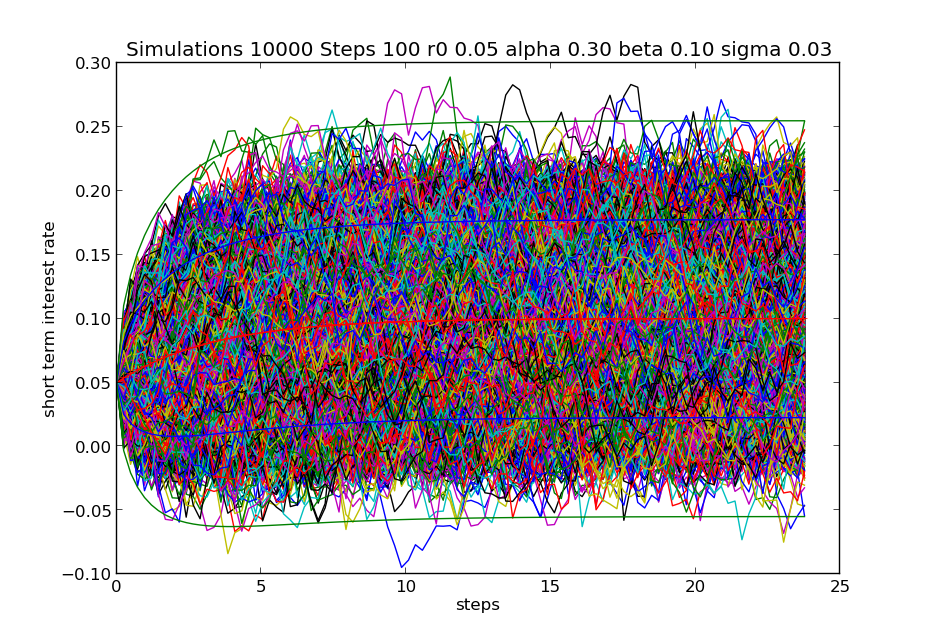
\includegraphics[bb=0 0 672 459,scale=0.5]{monte_carlo_simulation_interestrates.png}
 % monte_carlo_simulation_interestrates.png: 933x638 pixel, 100dpi, 23.70x16.21 cm, bb=0 0 672 459
\end{center}

